\documentclass[a4paper]{article}
\usepackage{graphicx}

\begin{document}

\title{Measure of unevenness in human genomes, described as a self-affine phase transition in a ''spin-chain'' model.}

\author{Sergey Feranchuk \\{\small(self-employed; residence: Smolensk, Russia; e-mail: feranchuk@gmail.com)}}

\maketitle

\section{Abstract}

Non-Gaussian distribution of polymorphic positions across a genome can substantially influence the results of any approach to molecular evolution based on a ''classical'' probability model. The infinite dispersion of non-Gaussian perturbations is a challenge in an attempts to accept it in a probability-based model of evolution.

Here a model is proposed where non-Gaussian distribution is introduced to an exact solution of the ''Ising model''; it describes a behavior of one-dimensional chain of spins in an approaching to a phase transition. The distribution of fragments which are identical between two genomes is similar to distribution of islands of spins with the same orientation, in the model where non-integer dimension is introduced.


Application of this model allows to compare the relative contributions of non-Gaussian perturbations for pairs of human genomes from different
ethnic groups. An evolution of the three human races in a most compact presentation is considered, rates of development on the separated stages
of the evolution are assumed to be proportional to a value of relative unevenness between the appropriate groups of genomes. In the resolved
model, the meaningful details of the separation between Asian and European races are clarified, in a period around ten thousands years ago; a
particular viewpoint to the separation of the African race is also presented.

\section{Introduction}

The issues about an unevenness of a genome arose in particular in a distribution of coverage of sequencing
reads mapped to a genome [1]. There, the deviations of a reads coverage from a ''classical'' Lange-Waterman
model, which was constructed following a Poisson distribution for short genome fragments, refects some features of self-affinity for most frequent genome fragments, in addition to the previously observed over-dispersion of a ''Poisson'' peak. There, the effect was observed stably in several analyzed genomes and is to be treated as a robust enough phenomenon to be discovered further and in deep.

The features of self-affinity in DNA sequences were detected at the very early days of the genomics, in a classical work of Peng et al. [2]; a definition of the fractal dimension for the one-dimensional series was proposed there, and DNA sequences were a model of ''fractal''-like series.
The self-affinity features in a phenomenon imply an influence of perturbations with infinite dispersion, or a presence of a so-called ''fat-tail'' in their probability distribution, and these features are difficult to detect and describe. 

Here, an approach is proposed to detect and apply a measure to these ''perturbations'' focusing on the mentioned phenomenon which was observed
in coverage distributions. A relevance of a proposed research is demonstrated on a model of evolution of humans restored from some of the present-day human genomes; confusions which are accumulated in solving of this scientific problem were in fact a motif to drive out the research.

\section{Methods}

Self-affinity features are a property of ''transitional'' period, and a description of these features is borrowed from approaches to a so-called ''Ising model'', the model
where a phase transition in a mutual orientations of spins in a crystal is explained. 
A heating of magnetic crystal leads to abrupt disappearance of magnetic momentum, and an approximation of this
phenomenon is simulated in the Ising model. In a very simplified form, the interactions in crystal are presented
there as an increase of energy if two spins in a linear chain are oriented in the same direction, and a critical
temperature of phase transition (Tc) is derived from a strength of these interactions (''coupling constant'').

The cooling lead in turn to a sudden appearance of magnetic momentum, and a decrease of a temperature
close to a critical temperature leads to accumulation of ''islands'', long enough fragments where
spins are oriented in the same order. Ordered fragments in a one-dimensional spin chain can be compared to identical fragments of genome sequences, and a distribution of these fragments allows to describe there the features of self-affinity. 

In the context of statistical physics, an expression for the probability of island of length k was presented in [3], as an applied case of the so-called ''Landau-Zener transition'': $p(k,\tau)  \sim e^{−\tau k^2}$


This is a point where a distribution with infinite dispersion can be introduced, assuming that a power coefficient 2 in this Gaussian-like distribution is substituted
to some floating power coefficient D < 2, a dimension of ''intrinsic'' self-affinity of the under-laid process. The model constructed above depends on the two
flexible parameters, intrinsic dimension D and a parameter $\tau$ , a rate of cooling, or a rate of approaching to a transitional phase. This model allows to explain over-
dispersion of the genome coverage distributions mentioned above (fig. 1) and to fit the parameters to a measure of unevenness of human genomes, trying to
reconstruct most precisely their evolution. The distribution of ''islands'' for human genomes can be obtained as distribution of lengths of completely
identical fragments in the genomes; lists of polymorphic positions from ''1000 genomes'' project [4] were used as a representation of genomes. Similar distribution of
fragment sizes is observed for this data (fig. 2A). The clusters for the three races are clearly seen for both genetic distance and for tails of ''island'' sizes
in genome-genome comparison (fig. 2B). To interpret this, higher unevenness relatively to same genetic distance means higher ''equilibration rate'', higher mutation rates, and a lesser slope of a fitting line.

\section{Results}

For the two independent populations, the distance does not depend of heterogeneity in populations; a simple model of exponential development can provide a dependency of average genetic distance within population.


The simplified model of evolution of human ethnic groups is shown in fig. 3, and for further consideration it was reduced to just clarify a separation between three human races. In this case, the model can be further reduced to a system of equations (2). The events which are assumed here as events of separation between races are (a) separation between modern Asians and modern Europeans, which happened nearly just after an expansion to America, about ten thousands years ago; and (b) expansion of modern humans to Eurasia, about fifty thousands years ago.


In the provided equations the mutation rate $r$ for humans is supposed to be fixed, conventionally it is accepted to be about $10^{-9}$
substitutions per nucleotide per year. The two types of averaged similarities within a race and between races which are clearly seen in fig 2 are provided in table 1 in the appropriate units.


The mutation rate $10^{-9}$ per nucleotide per year can be transformed as 3 per genome per year = 3000 per
genome per t.y., 3000 mutations per 700000 SNP, so that r in the equations above should be about 0.004.
Having a requirement that $p_0 >= 0$, the $r$ should be less than 0.0029. Rates of development are assumed to be unknown,
what is only known is a dependency between a rate of development and a linear coefficient $m$. Values of
$b_a, b_e, b_A, p_{ae}, k_{ae}$ which are attributes of a passed history are also assumed to be unknown.


For a marginal but the most confident assumption, $p_0 = 0, p_{ae} = 0.21, kA = 1.65$ and $k_{ae} = 1.81$. Unevenness in a comparison between groups is a weighted
average of evolutionary paths from a time of separation, so that if $kA \sim mA$, $ke \sim me$, then $k_{ae} \sim (m_{Ae}T + mA(T + t) + m_e t)/2(T + t)$; $k_{ae} \approx 0.0141$. Following a log-linear approximation, $k_a$ and $k_e$, for modern Asians and Europeans, should be about 1.74 and 1.76.

The genetic diversity of Asians in a time of separation is than estimated as 0.15, much lower than a pool of genotypes just before the separation ($p_{ae} = 0.21$). For Europeans, the pool of genotypes was wider, about 0.20.

What is known is that Eurasia is a continent with good communications, and that it was populated
mostly by ancestors of present-day Asian race before the time of last separation, or ''crash'', in better words.
It is also known that ancestors of modern Europeans become to expand to Europe mostly after that ''crash'',
developing slowly before it somewhere in an area of central Asia mountains. The wide expansion to Eurasia,
for ancient pre-Asian race, was characterized, instead, by a substantive increase of genome unevenness. Some
of it now is lost, some is kept in native Americans, and, for modern Asians, the instabilities in diverged
genomes were neutralized by a long enough period of a stable slow development after the crash.


\section{Conclusions}

Selection of individuals was almost the same as in [5], the difference with that model is that non-Gaussian features in genomes are considered here explicitly. This
have a substantial influence to a reconstructed history of the three human races. Dealing with self-affine phenomena is difficult and risky, but it by no way can be ignored in any of valuable challenges to a present-day
science.

\section{Formal declarations}

\begin{itemize}

\item The author has no competing interests in the scientific business.

\item No funding was acquired for the provided research. 

\item Acknowledgements are intentionally omitted.

\item Source codes of the scripts and intermediate data are deposited to zenodo.org (10.5281/zenodo.4362224).

\end{itemize}

\section{References}

\begin{enumerate}

\item Kuzmin D., et al., Stepwise large genome assembly approach: A case of Siberian larch, BMC Bioinformatics, 2019.

\item Peng C.-K., et al., Mosaic organization of DNA nucleotides, Phys.Rev., 1994.

\item Dziarmaga J., Dynamics of quantum phase transition : exact solution in quantum Ising model. arxiv.org, 2005.

\item Durbin R., et al., An integrated map of genetic variation from 1.092 human genomes, Nature, 2012.

\item Schiffels S., Durbin R., Inferring human population size and separation history from multiple genome sequences. Nature Genetics, 2014.

\end{enumerate}

\newpage

\section*{Figure 1}

\vskip 10pt

\includegraphics[width=0.8\textwidth]{fig1.png}

\vskip 15pt

(A) Simulation of over-dispersion effect in a genome following modified Ising model
of islands in a chain of spins. Here, $D$ = 1.9, $\tau$ = 0.0005, number of spins $N$ = 200. Dashed line,
$ke^{−\tau k^2}$ , emulates an ordinary Poisson distribution, $\tau$ is the same. (B) Dependency between
estimated fitting coefficient, average of distribution, and underlying closeness to ''phase transition''.

\newpage 

\section*{Figure 2}

\vskip 10pt

\includegraphics[width=0.99\textwidth]{fig2a.jpg}

\begin{minipage}[ht]{0.35\textwidth}
    \includegraphics[width=0.99\textwidth]{fig2b.jpg}
\end{minipage}
\hfill
\begin{minipage}[ht]{0.35\textwidth}
    \includegraphics[width=0.99\textwidth]{fig2c.jpg}
\end{minipage}

\vskip 15pt

(A) Distribution of fragments sizes in human genomes in a pairwise comparison. (B,C)
Measures of closeness between genomes: genetic distance (B) and unevenness of fragment sizes
(C). Here, races are, from left to right, from bottom to top: Asia, Mexico, Europe, India, Africa.

\newpage

\section*{Figure 3}

\vskip 10pt

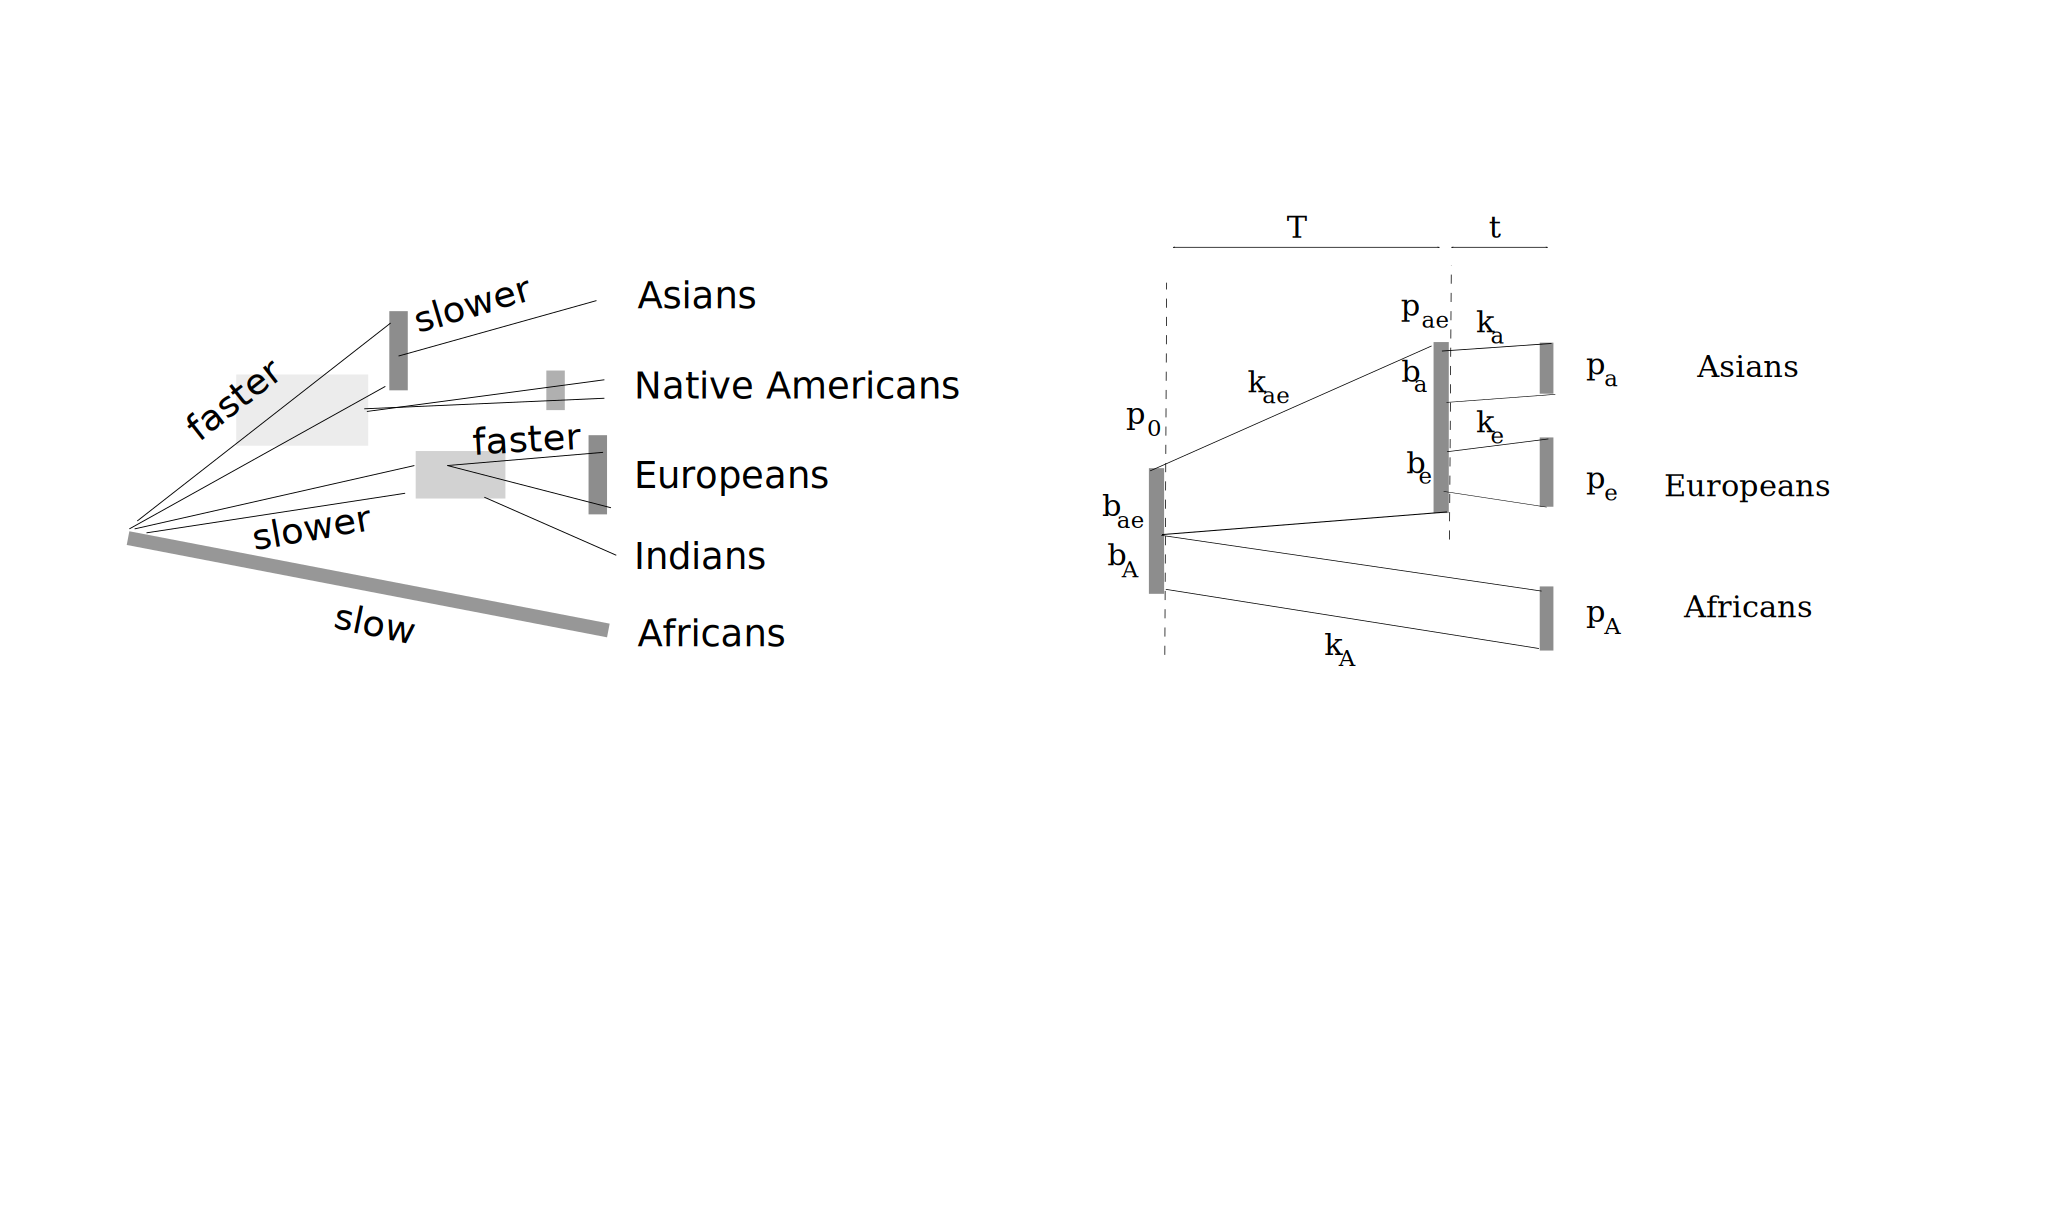
\includegraphics[width=0.9\textwidth]{fig3.png}

\vskip 15pt

Simplified presentation of human evolution. $p_a, p_e,$ ... - heterogeneity of genomes within a communicating group; $d_{ae},$ ... - distance
between genomes of separated groups; $b_e, b_a,$ ... relative heterogeneity of a group in the events of separation between groups. $k_a, k_e,$ ... - rates of
''exponential'' development.

\newpage

\section*{Table 1}

Approximated averaged similarities between human races and within a race, accordingly to the detailed chart in Fig. 2.

\vskip 5pt

\begin{tabular}{cccc}
 Races & &''unevenness'' $m$ &genetic distance $p$\\
\hline
Europe&Europe&0.0138&0.25\\
Europe&Asia&0.0144&0.27\\
Asia&Asia&0.0137&0.22\\
Europe&Africa&0.0152&0.29\\
Asia&Africa&0.0153&0.29\\
Africa&Africa&0.0131&0.24\\
\hline
\end{tabular}

\end{document}
